% !TEX root =  podc-submission.tex

\section{Analysis}
In this section, we analyze the number of \nf{CAS} invocations and the time complexity of our algorithm.
\begin{proposition}
An \nf{Enqueue} or \nf{Dequeue} operation does at most $14\log p$ \nf{CAS} operations.
\end{proposition}
\begin{proof}
  In each level of the tree  \nf{Refresh} is invoked at most two times, and every \nf{Refresh} invokes at most seven \nf{CAS}es, one in Line \ref{cas} and two from each \nf{Advance} in Line \ref{helpAdvance} or \ref{advance}.
\end{proof}

\begin{lemma}[\nf{DoublingSearch} Analysis]\label{dsearchTime}
If the \nf{element} enqueued by $E_i(root,b)=E_e(root)$ is the response to some \nf{Dequeue} operation in \nf{root.blocks[$end$]}, then \nf{DoublingSearch($e$, $end$)} takes $O\big(\log ( \nf{root.blocks[$b$].size}+ \nf{root.blocks[$end$].size})\big )$ steps.
\end{lemma}
\begin{proof}
First we show $end - b -1\leq 2 \times \nf{root.blocks[$b-1$].size}+\nf{root.blocks[$end$].size}$. There can be at most \nf{root.blocks[$b$].size}  \nf{Dequeue}s in \nf{root.blocks[$b+1\cdots end-1$]}; otherwise all elements enqueued by \nf{root.blocks[$b$]} would be dequeued before \nf{root.blocks[$end$]}. Furthermore, in the execution of queue operations in the linearization ordering, the size of the queue becomes \nf{root.blocks[$end$].size} after the operations of \nf{root.blocks[$end$]}. The final size of the queue after \nf{root.blocks[$1\cdots end$]} is \nf{root.blocks[$end$].size}. After an execution on a queue, the $size$ of the queue is greater than or equal to $\#enqueues -\#dequeues$ in the execution. We know the number of dequeues in \nf{root.blocks[$b+1\cdots end-1$]} is less than \nf{root.blocks[$b$].size}, therefore in \nf{root.blocks[$b+1\cdots end-1$]} there cannot be more than $\nf{root.blocks[$b$].size} + \nf{root.blocks[$end$].size}$ \nf{Enqueue}s. Overall there can be at most $2 \times\nf{root.blocks[$b$].size}+ \nf{root.blocks[$end$].size}$ operations in \nf{root.blocks[$b+1\cdots end-1$]} and since from Line \ref{addOP} we know that the \nf{num} field of every block in the tree is greater than 0, each block has at least one operation, so there are at most $2 \times\nf{root.blocks[$b$].size}+ \nf{root.blocks[$end$].size}$ blocks in between \nf{root.blocks[$b$]} and \nf{root.blocks[$end$]}. So, $end-b-1\leq 2 \times\nf{root.blocks[$b$].size}+\nf{root.blocks[$end$].size}$.

Thus, the doubling search reaches \nf{start} such that the \nf{root.blocks[start].sum\sub{enq}} is less than $e$ in $O \big(\log(\nf{root.blocks[$b$].size}+\nf{root.blocks[$end$].size})\big)$ steps. See Figure \ref{fig::doubling}. After Line \ref{dsearchEnd}, the binary search that finds $b$ also takes $O\big(\log(\nf{root.blocks[$b$].size}+\nf{root.blocks[$end$].size})\big)$. Next, \nf{i} is computed via the definition of \nf{sum\sub{enq}} in constant time (Line \ref{DSearchComputei}).
\end{proof}
\begin{figure}[hbt]  
  \center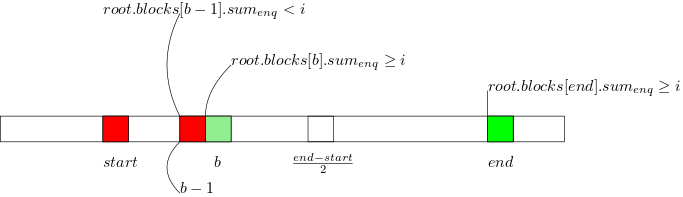
\includegraphics[width=6in]{pics/doubling.png}
  \caption{Distance relations between \nf{start}$,b,end$.}
  \label{fig::doubling}
\end{figure}

\begin{lemma}[Worst Case Time Analysis] \label{enqDeqTime}
The worst case number of steps for an \nf{Enqueue} is $O(\log^2 p)$ and for a \nf{Dequeue}, is $O(\log^2 p + \log q_e+ \log q_d)$, where $q_d$ is the size of the queue when the \nf{Dequeue} is linearized and $q_e$ is the size of the queue at the time the response of the \nf{Dequeue} is linearized.
\end{lemma}
\begin{proof}
\nf{Enqueue} consists of creating a block and appending it to the tree. The first part takes constant time. To propagate the operation to the root the algorithm tries at most two \nf{Refresh}es in each node of the path from the leaf to the root (Lines \ref{firstRefresh}, \ref{secondRefresh}). We can see from the code  that each \nf{Refresh} takes a constant number of steps and does $O(1)$ \nf{CAS}es. Since the height of the tree is $\Theta(\log p)$, \nf{Enqueue} takes $O(\log p)$ steps.

A \nf{Dequeue} creates a block whose \nf{element} is \nf{null}, appends it to the tree, computes its rank among non-null dequeues, finds the corresponding enqueue and returns the response. The first two parts are similar to an \nf{Enqueue} operation and take $O(\log p)$ steps. To compute the rank of a \nf{Dequeue} in $D(n)$, the \nf{Dequeue} calls \nf{IndexDequeue()}. \nf{IndexDequeue} does $O(1)$ steps in each level which takes $O(\log p)$ steps. If the response to the \nf{Dequeue} is \nf{null}, \nf{FindResponse} returns \nf{null} in $O(1)$ steps. Otherwise, if the response to a dequeue in \nf{root.blocks[end]} is in \nf{root.blocks[b]} the \nf{DoublingSearch} takes $\Theta(\log$(\nf{root.blocks[b].size+root.blocks} \nf{[end].size}) by Lemma~\ref{dsearchTime}, which is $O(\log q_e+\log q_d)$. Each search in \nf{GetEnqueue()} takes $O(\log p)$ steps since there are at most $p$ subblocks in a block (Lemma \ref{subBlocksBound}), so \nf{GetEnqueue()} takes $O(\log^2 p)$ steps.
\end{proof}


\begin{lemma}[Amortized Worst-case Analysis]
The amortized number of steps for an \nf{Enqueue} or \nf{Dequeue} is $O(\log^2 p + \log q)$,  where $q$ is the size of the queue when the operation is linearized.
\end{lemma}
\begin{proof}
If we split the \nf{DoublingSearch} time cost between the corresponding \nf{Enqueue} and \nf{Dequeue}, each operation takes $O(\log^2 p +q)$ steps.
\end{proof}

\begin{observation}
    If the maximum number of concurrent processes at any time in an execution is $c$, then the amortized worst-case step complexity is $O(\log p\log c + \log q)$ per operations. Furthermore, in a sequential, execution where $c=1$, the step complexity of our algorithm is $\Theta(\log p + \log q)$ per operation.
\end{observation}
\begin{proof}
    The analysis is similar to the two previous Lemmas, but by Lemma \ref{subBlocksBound} each \nf{BinarySearch} in each call of \nf{GetEnqueue} takes $O(\log c)$ steps.
\end{proof}

\begin{theorem}
The queue implementation is wait-free.
\end{theorem}
\begin{proof}
To prove the claim, it is sufficient to show that every \nf{Enqueue} and \nf{Dequeue} operation terminates after a finite number of its own steps. This is directly concluded from Lemma \ref{enqDeqTime}.
\end{proof}
